\documentclass{tikzposter} %Options for format can be included here

\usepackage{todonotes}

\usepackage[tikz]{bclogo}
\usepackage{lipsum}
\usepackage{amsmath}

\usepackage{booktabs}
\usepackage{longtable}
\usepackage[absolute]{textpos}
\usepackage[it]{subfigure}
\usepackage{graphicx}
\usepackage{cmbright}
%\usepackage[default]{cantarell}
%\usepackage{avant}
%\usepackage[math]{iwona}
\usepackage[math]{kurier}
\usepackage[T1]{fontenc}


%% add your packages here
\usepackage{hyperref}
% for random text
\usepackage{lipsum}
\usepackage[english]{babel}
\usepackage[pangram]{blindtext}

\colorlet{backgroundcolor}{blue!10}

% Title, Author, Institute
\title{Group 00 hypothetical organisation}
\author{Sarah Sun}
\institute{Deakin University, AU}
%\titlegraphic{logos/tulip-logo.eps}

%Choose Layout
\usetheme{Wave}

\definebackgroundstyle{samplebackgroundstyle}{
	\draw[inner sep=0pt, line width=0pt, color=red, fill=backgroundcolor!30!black]
	(bottomleft) rectangle (topright);
}
%
\colorlet{backgroundcolor}{blue!10}

\begin{document}
	
	
	\colorlet{blocktitlebgcolor}{blue!23}
	
	% Title block with title, author, logo, etc.
	\maketitle
	
	\begin{columns}
		% FIRST column
		\column{0.5}% Width set relative to text width
		
		%%%%%%%%%% -------------------------------------------------------------------- %%%%%%%%%%
		%\block{Main Objectives}{
		%  	      	\begin{enumerate}
		%  	      	\item Formalise research problem by extending \emph{outlying aspects mining}
		%  	      	\item Proposed \emph{GOAM} algorithm is to solve research problem
		%  	      	\item Utilise pruning strategies to reduce time complexity
		%  	      	\end{enumerate}
		%%  	      \end{minipage}
		%}
		%%%%%%%%%% -------------------------------------------------------------------- %%%%%%%%%%
		
		
		%%%%%%%%%% -------------------------------------------------------------------- %%%%%%%%%%
		\block{Introduction}{
			Not only does it embody all the creative energy.
			Spirit of TULIP-Lab, it’s a “learning environment” on which the tourism
			and hospitality students are trained for future hoteliers.\\
			Improve their potential customers’ online experience,and help their Market
			Promotion Division toidentify potential customers and their behaviour patterns
			\item{·In the past two decades}
			\item{·the Web server of Hotel TULIP has logged all the web traffic to the hotel
				website.}
			\item{·Stored large amount of data related to the use of various web pages}
		}
		%%%%%%%%%% -------------------------------------------------------------------- %%%%%%%%%%
		
		
		%%%%%%%%%% -------------------------------------------------------------------- %%%%%%%%%%
		\block{Process}{
			\begin{itemize}
				\item
				Performing data clean-up: removing missing and Nan values.
				\item
				Bar chart of user hits on the website by hour.
				\item
				Analysis of the protocol status of users visiting the site to determine the comparison of first and second visits by users.
				\item
				The ip of the user logging into the website is analysed. Statistics from national level and city level.
			\end{itemize}
		}
		%%%%%%%%%% -------------------------------------------------------------------- %%%%%%%%%%
		
		
		%%%%%%%%%% -------------------------------------------------------------------- %%%%%%%%%%
		
		%\note{Note with default behavior}
		
		%\note[targetoffsetx=12cm, targetoffsety=-1cm, angle=20, rotate=25]
		%{Note \\ offset and rotated}
		
		% First column - second block
		
		
		%%%%%%%%%% -------------------------------------------------------------------- %%%%%%%%%%
		\block{Data visualization-bar chart}{
			The data obtained will be analysed using bar and sector charts. It is very clear what proportion of the total is accounted for by each component.
			%    1) Group Feature Extraction,
			%    2) Outlying Degree Scoring, and
			%    3) Outlying Aspects Identification.
			
			\begin{tikzfigure}%[Overall architecture of \emph{GOAM} algorithm]
				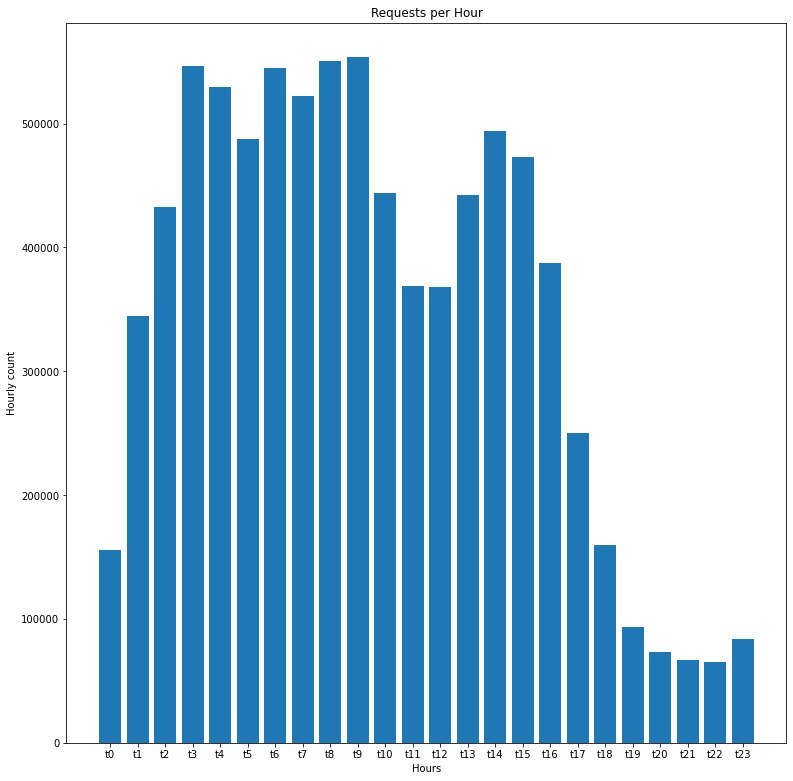
\includegraphics[width=1\linewidth]{figures//ll1.png}
				%    \missingfigure[figcolor=white]{Testing figcolor}
			\end{tikzfigure}
		}
		%%%%%%%%%% -------------------------------------------------------------------- %%%%%%%%%%
		
		
		% SECOND column
		\column{0.5}
		%Second column with first block's top edge aligned with with previous column's top.
		
		%%%%%%%%%% -------------------------------------------------------------------- %%%%%%%%%%
		\block{Data visualization-pie char}{
			\begin{description}
				\item
				The protocol state of the page that the user accesses.
			\end{description}
			
			\begin{tikzfigure}%[Overall architecture of \emph{GOAM} algorithm]
				% \missingfigure[figcolor=white]{Testing figcolor}
				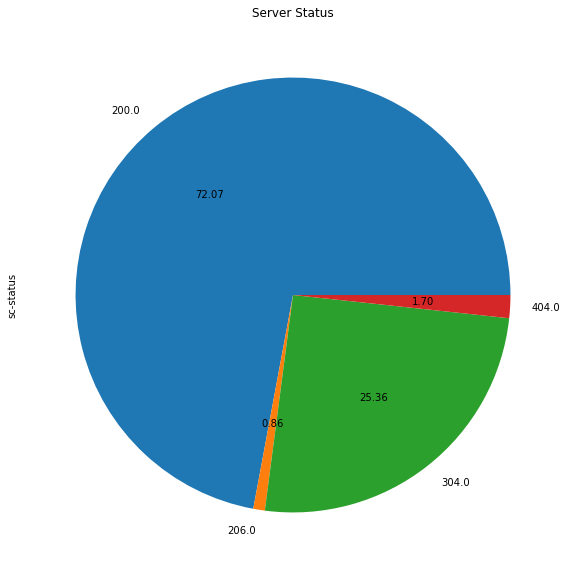
\includegraphics[width=0.4\linewidth]{figures//ll2.png}
				Six million people were the most successful.
				In second place is rendering 304, which means the server has a cache for the web page.
				This proves that the user has visited the site for the second or more times.
			\end{tikzfigure}
			
			\begin{tikzfigure}%[Overall architecture of \emph{GOAM} algorithm]
				% \missingfigure[figcolor=white]{Testing figcolor}
				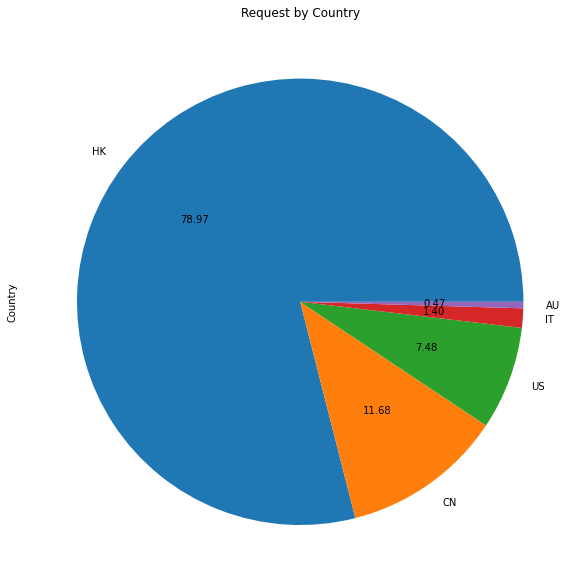
\includegraphics[width=0.4\linewidth]{figures//ll3.png}
				Want to know the possibilities of the location of potential users. The first is the country. Hong Kong, China and the USA were found to be the top three countries visited. Hong Kong is in the majority, so it is possible to re-market mainly to these three countries.
			\end{tikzfigure}
			\begin{tikzfigure}%[Overall architecture of \emph{GOAM} algorithm]
				% \missingfigure[figcolor=white]{Testing figcolor}
				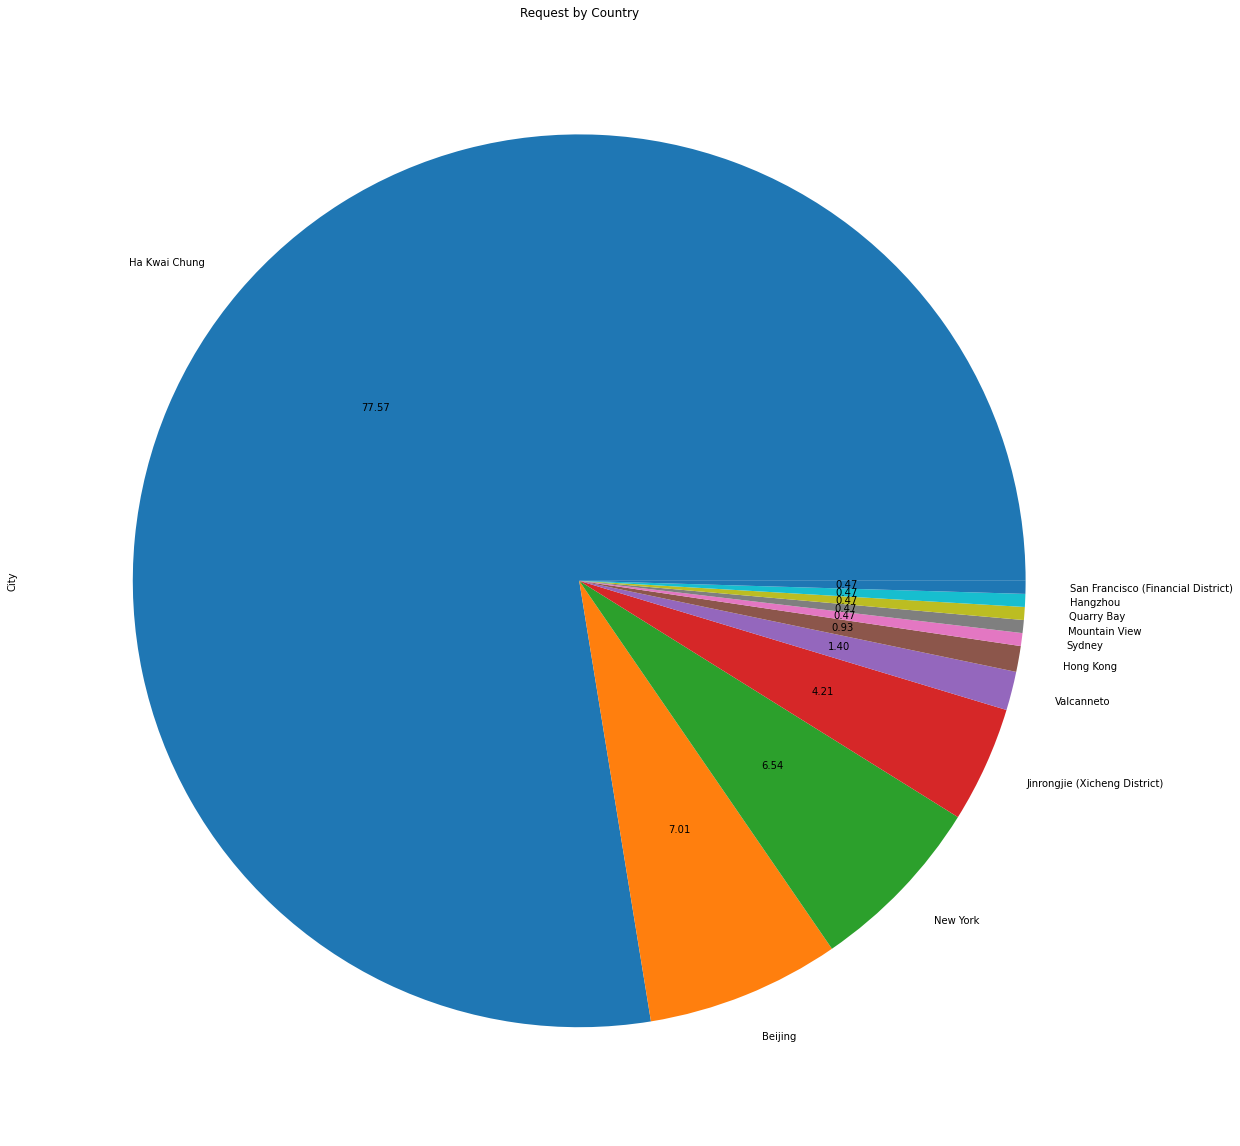
\includegraphics[width=0.4\linewidth]{figures//ll4.png}
				It is found that the first-tier cities in these three countries are the main visitors, such as Beijing in China and New York in the United States.
			\end{tikzfigure}
		}
		
		
		
		% Second column - second block
		%%%%%%%%%% -------------------------------------------------------------------- %%%%%%%%%%
		\block[titlewidthscale=1, bodywidthscale=1]
		{Conclusion}
		{
			\begin{description}
				\item[Definite purpose]
				What information is held in the dataset and what can it be used for
				
				\item[Data cleaning]
				There should be standards for cleaning and organising data, cleaning up nan and missing data, standardising tables.
				
				\item[Data visualization]
				It is important to choose the right visual representation of data that is intuitive and highlights the key points of the report.
			\end{description}
		}
		%%%%%%%%%% -------------------------------------------------------------------- %%%%%%%%%%
		
		
		% Bottomblock
		%%%%%%%%%% -------------------------------------------------------------------- %%%%%%%%%%
		
		
		%\note[targetoffsetx=8cm, targetoffsety=-10cm,rotate=0,angle=180,radius=8cm,width=.46\textwidth,innersep=.1cm]{
		%Acknowledgement
		%}
		
		%\block[titlewidthscale=0.9, bodywidthscale=0.9]
		%{Acknowledgement}{
		%}
		%%%%%%%%%% -------------------------------------------------------------------- %%%%%%%%%%
		
	\end{columns}
	
	
	%%%%%%%%%% -------------------------------------------------------------------- %%%%%%%%%%
	%[titleleft, titleoffsetx=2em, titleoffsety=1em, bodyoffsetx=2em,%
	%roundedcorners=10, linewidth=0mm, titlewidthscale=0.7,%
	%bodywidthscale=0.9, titlecenter]
	
	%\colorlet{noteframecolor}{blue!20}
	\colorlet{notebgcolor}{blue!20}
	\colorlet{notefrcolor}{blue!20}
	\note[targetoffsetx=-13cm, targetoffsety=-12cm,rotate=0,angle=180,radius=8cm,width=.96\textwidth,innersep=.4cm]
	{
		\begin{minipage}{0.3\linewidth}
			\centering
			
\includegraphics[width=24cm]{logos/tulip-wordmark.eps}
		\end{minipage}
		\begin{minipage}{0.7\linewidth}
			{ \centering
				The $11^{th}$ International Conference on Knowledge Science,
				Engineering and Management (KSEM 2018),
				17-19/08/2018, Changchun, China
			}
		\end{minipage}
	}
	%%%%%%%%%% -------------------------------------------------------------------- %%%%%%%%%%
	
	
\end{document}

%\endinput
%%
%% End of file `tikzposter-template.tex'.
